   
\section{Methodology}
\subsection{Data Imbalance}

The initial issue faced when starting to attempt to build a prediction model, was how to split the continuous variables supplied by the EmoBank dataset into discrete categories.

An initial look at the data shows that there is a large number of sentences represented with values a neutral area, and very few representing the extreme cases, as shown in Figure \ref{dist:vad}.

The simplest way to initially categorise the data is to round to the nearest whole number, but as shown in Figure \ref{dist:5cat}, the extreme classes are not well represented, and would prove very difficult to train a model off. Having 5 discrete classes for each dimension also provides more detail than is probably necessary for the task at hand, so can be simplified.

\begin{figure}[h]
\caption{Graph showing data distribution when split into five classes}
\centering
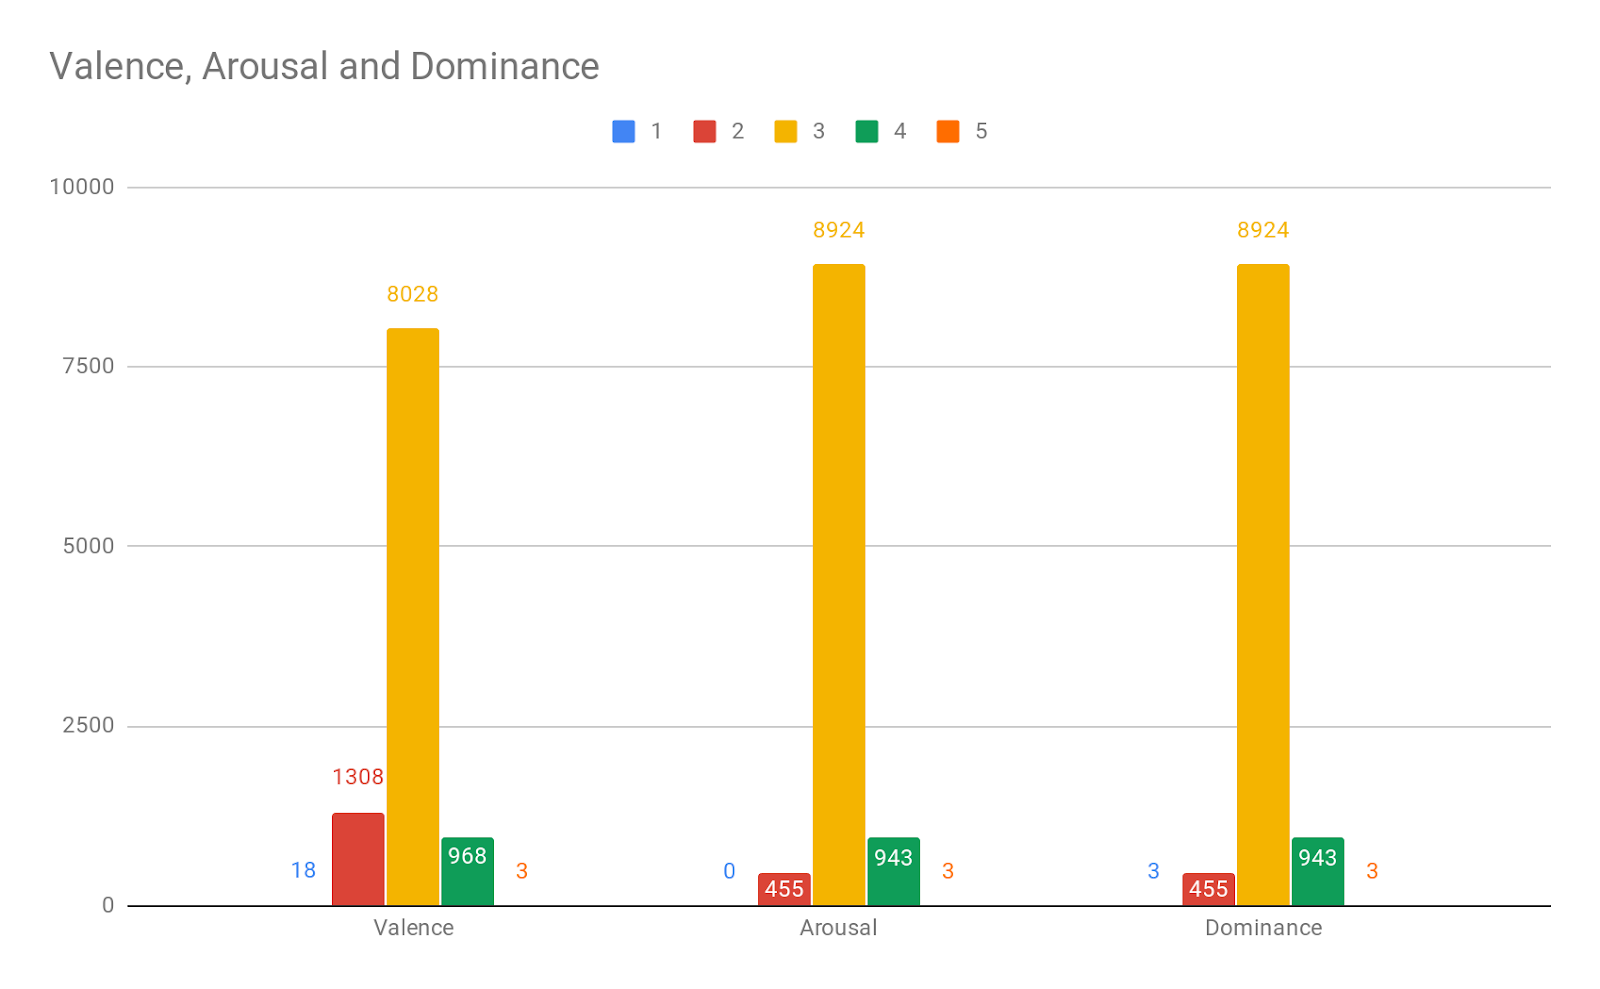
\includegraphics[scale=0.3]{graphs/5catDist.png}
\label{dist:5cat}
\end{figure}

Splitting each dimension up into positive or negative values is also is an option, allowing an easier comparison to other work which generally does this. The issue here is that the data imbalance is still very great, particularly with the Arousal and Dominance dimensions, as shown in Figure \ref{dist:bin}.

\begin{figure}[ht]
\caption{Graph showing data distribution when split into binary positive and negative classes}
\centering
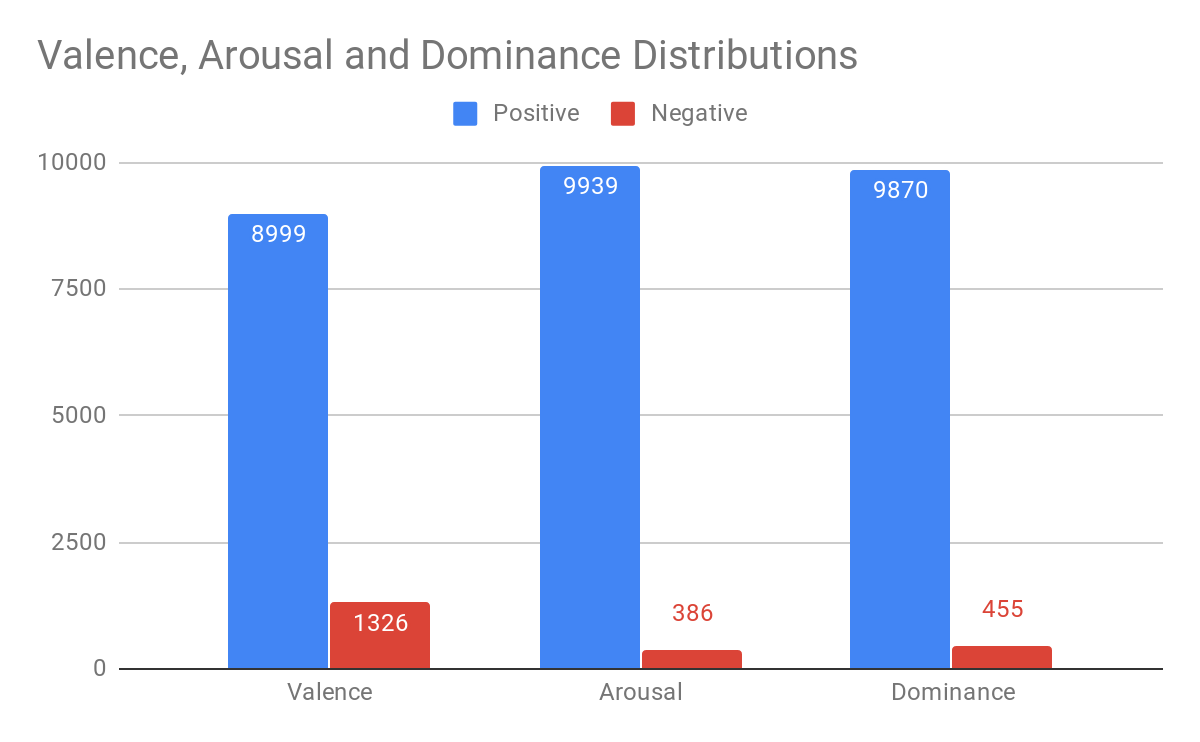
\includegraphics[scale=0.25]{graphs/binaryDist.png}
\label{dist:bin}
\end{figure}

A middle ground can be found when splitting the data into positive, neutral and negative classes, as even though there is still a data imbalance there, it is less severe, and this is chosen as how to represent the data moving forward, shown in Figure \ref{dist:tri}.

\begin{figure}[H]
\caption{Graph showing data distribution when split into positive, neutral negative classes}
\centering
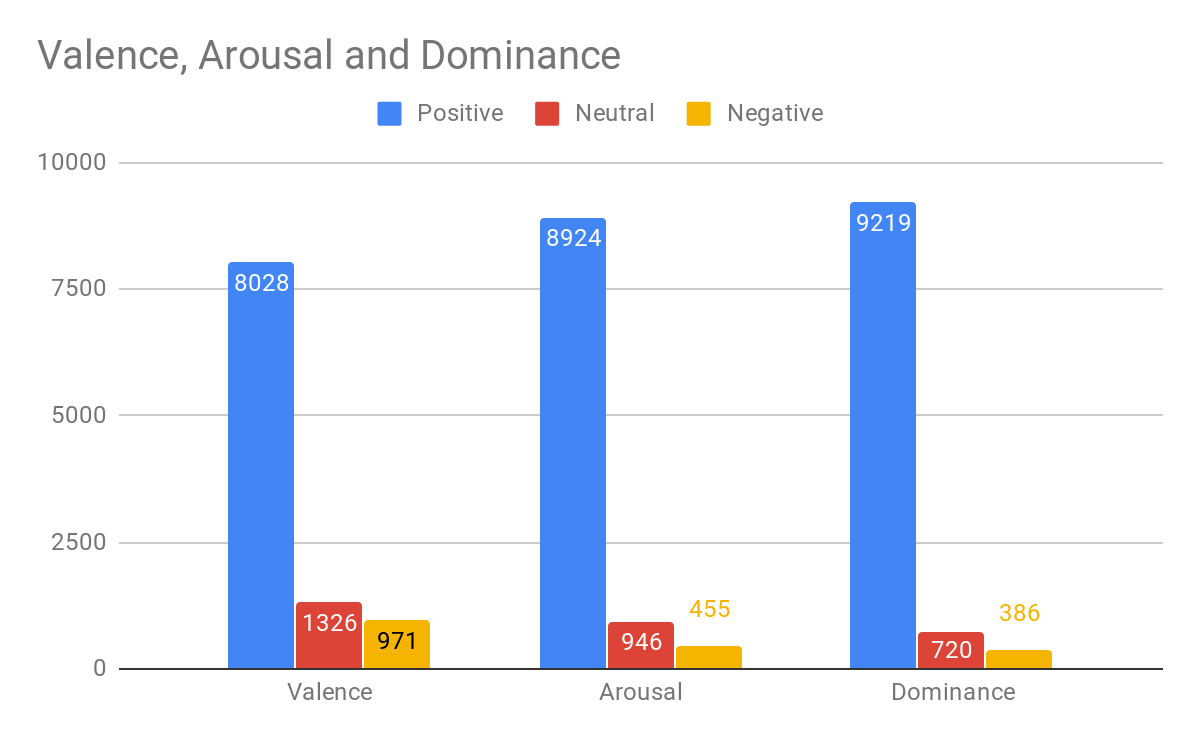
\includegraphics[scale=0.3]{graphs/nonBinaryDist.png}
\label{dist:tri}
\end{figure}

\pagebreak


\subsection{Hypothesis Tests}

To argue for each of the decisions made when building the final model, a hypothesis test with a 90\% confidence level will be carried out.

Due to the imbalance in the data, a prediction accuracy cannot be used for comparing the models. This is because the majority class dominates, with it being the most likely to be predicted as there are simply more examples available \cite{al2015applied}, heavily biasing the accuracy results.

For each investigation that is carried out, a confusion matrix is be produced as shown in Table \ref{conmat}, so that proper analysis of the results can be made.

\begin{table}
\centering
\caption{Structure of produced confusion matrices}
\begin{tabular}{ |p{3cm}|p{3cm}|p{3cm}|p{3cm}|p{3cm}| }
 \hline
  & \multicolumn{3}{|c|}{Predicted} &\\
 \hline
   Actual & Negative & Neutral & Positive &\\
    \hline
    Negative &  True Negative   &  False Negative  & False Negative & Total Negative\\
    Neutral & False Neutral & True Neutral&  False Neutral & Total Neutral \\
    Positive & False Positive & False Positive &  True Positive & Total Positive\\
    \hline
    & Total Predicted Negative & Total Predicted Neutral & Total Predicted Positive & \\
 \hline
\end{tabular}
\label{conmat}
\end{table}

The F1 score of the prediction model is used in the hypothesis tests. The F1 score is the weighted average of the Precision and Recall of a model, which are defined as follows: 

$$ F1 = 2 * \frac{Precision * Recall}{Precision + Recall} $$

And then the precision and recall values can be calculated as follows:

$$ Precision_{Class} = \frac{True_{Class}}{Total Predicted_{Class}} $$

$$ Recall_{Class} = \frac{True_{Class}}{Total_{Class}} $$

Each of the experiments are run with stratified K-Fold validation, with the data from each fold being used for the hypothesis test comparisons, using 10 folds. The folds are stratified so that the representation of each class remains the same in each fold which is needed due to the large data imbalance \cite{kohavi1995study}.

Using this score instead of the accuracy gets rid of the class bias, and in this case it is calculated using the micro-average of the K-Folds. The micro average aggregates the contributions of each class so that any imbalance can be mitigated.

The hypothesis test that will be performed on the data will be the Wilcoxon Signed-Rank Test, since the comparison between the data will be on two related samples, and the data cannot be assumed to be normally distributed within the folds, meaning that this is the best test to be using in this case \cite{wilcoxon1970critical}.

\subsection{Lexicon Analysis}

For the bag-of-words model, we will calculate the confusion matrix and then the F1 score by totalling up the values for each sentence over the Emobank dataset, and then comparing the two results, the calculated values, and the ones given in Emobank sample. The values are calculated by looking up each word in the bag-of-words dataset \cite{wordsData}.

To get the words from the EmoBank dataset into a state where they are most likely to be found within the lexicon datase, some natural language processing needs to be done on the data, using the NLTK \cite{NLTKBook} library to stem the words, returning words to their root form.

For example, the word "Fishing" would be reduced to the word "Fish" after being stemmed. 

As we can see from Figure \ref{lexiconGraph}, the average values for the Arousal are much lower across the bag-of-word dataset, and this is reflected in the F1 scores for each dimension that are returned from this lexicon based model:

\begin{table}
\centering
\label{lexicon:f1}
\caption{F1 scores for the 3 dimensions for the bag-of-words model}
\begin{tabular}{ |p{3cm}|p{3cm}|}
 \hline
  Dimension & F1 Score \\
 \hline
  Valence & 0.72\\
  Arousal & 0.08 \\
  Dominance & 0.80\\
 \hline
\end{tabular}

\end{table}

We can see that for the Valence and Dominance dimensions, this form of prediction performs quite well, and whether these scores can be further improved with machine learning methods will be interesting.

To explore why the Arousal dimension performs so badly, we can take a closer look at the generated confusion matrix, as shown in Table \ref{lexicon:a:conmat}. As we can see, most of the neutral data was predicted to be negative, which is definitely influenced by the trend in the bag-of-words dataset, where the average values for the Arousal are quite low. There are also no correctly predicted values in the positive class, which also contributes to the extremely low F1 score.

\begin{table}
\centering
\label{lexicon:a:conmat}
\caption{Confusion matrix for Arousal}
\begin{tabular}{ |p{3cm}|p{3cm}|p{3cm}|p{3cm}| }
 \hline
  & \multicolumn{3}{|c|}{Predicted} \\
 \hline
   Actual & Negative & Neutral & Positive \\
    \hline
    Negative &  313   &  10  & 0 \\
    Neutral & 7001 & 384 &  3 \\
    Positive & 656 & 83 &  0 \\

 \hline
\end{tabular}

\end{table}


It is also worth noting that the values in Table \ref{lexicon:a:conmat} do not cover the whole dataset either, due to instances when all of the words in the EmoBank sample cannot be found within the lexicon dataset. In this case there are around 1,500 sentences for which a VAD value could not be calculated, showing that this bag-of-words based method is far from optimal since all of the data cannot be analysed.

\subsection{Data Pre-processing (N-Gram and Feature selection)}

Following R. Kim's investigations into semantic analysis \cite{towardsDS}, an investigation into optimising the format for the data input is carried out. 

To be able to analyse the text, the sklearn CountVectorizer library is used to return a sparse matrix of the counts of each word in the input vocabulary, which then become the features for inputting into a machine learning classifier \cite{sklearn}.

From this we can also limit the number of features that we can take, with the number of features being the number of most popular N-Grams, and we can set the N-Gram range easily. 

The previous investigation only tried N-Gram values ranging up to trigram, but to ensure that this is an optimal result, the experiment will be carried out up to fourgram.

The range of features that was used previously was up to 10,0000 features because the results did not improve after this, but since we are using a different dataset, the number of features tested was increased until the resultant graph implied that the F1 score did not improve further. 

The model used to investigate how the F1 score varies as the inputs change will be a Logistic Regression model, as this has been shown to give the most promising results in previous work \cite{towardsDS}.

\begin{figure}[h]
\caption{Experimental Results for varying the number of features and values for N-Gram sequences}
\centering
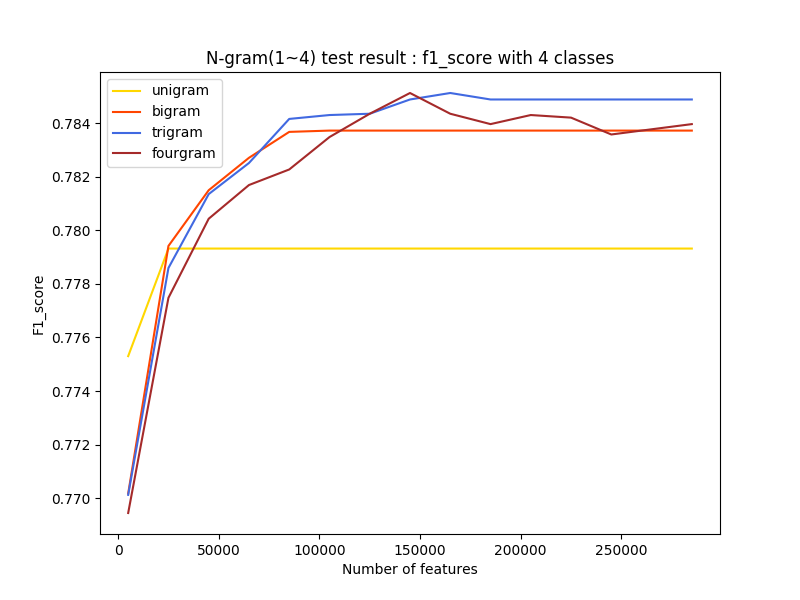
\includegraphics[scale=0.7]{graphs/nGramBinaryGraph300000.png}
\label{ngramGraph}
\end{figure}

As shown in Figure \ref{ngramGraph}, the F1 score improves as the N-Gram value increases up to a point, and the score also increases as the number of features does. An explanation of why the values for fourgram are generally less than for trigram, could be because the dataset is not that large and therefore predictions are less accurate as the relationships between the words cannot be properly established, so for our purposes we can leave out fourgram. It requires a significantly higher amount of processing time, as shown in Table \ref{ngram:time}. The values in Table \ref{ngram:time} are estimates calculated just to show the scale differences between the variables.


\begin{table}
\centering
\caption{Approximate Computation time for each N-Gram value.}
\label{ngram:time}
\begin{tabular}{ |p{3cm}|p{3cm}|}
 \hline
  N-Gram selection & Time (s) \\
 \hline
  unigram & 71\\
  bigram & 241\\
  trigram & 406\\
  fourgram & 1105 \\
 \hline
\end{tabular}

\end{table}
\pagebreak

\subsubsection{Hypothesis Tests} \todo{optimal way to show hypothesis test results?}

Using the trigram values to compare, the hypothesis test shows that the F1 score still increases after 85,000 features as shown below:

$$ H_0:  \textnormal{F1 score at 85,000 features is the same than at 165,000 features (the peak on the graph)}$$

$$ H_a: \textnormal{F1 score at 85,000 features is less than at 165,000 features} $$

Using the Wilcoxon rank sum test with 90\% confidence interval 
p = 0.08 so reject $H_0$

But the score for F1 does not increase significantly after 105,000, which is shown as follows:

$$H_0: \textnormal{F1 score at 105,000 features is the same than at 165,000 features} $$
$$H_a: \textnormal{F1 score at 105,000 features is less than at 165,000 features}$$

Using the Wilcoxon rank sum test with 90\% confidence interval 
p = 0.15 so reject $H_a$


We can conclude that the optimal number of features to use in the model is 105,000, and this value will be used in the rest of the investigations as to maximise the score of the resultant model. 


Using this value of 105,000 features, we can compare bigram and trigram results in the following test:

$$ H_0: \textnormal{F1 score of Bigram and Trigram is the same at 105,000 features} $$
$$ H_1: \textnormal{F1 score of Bigram is less than Trigram at 105,000 features} $$

Using the Wilcoxon rank sum test with 90\% confidence interval 
p = 0.10

This value is just on the margin, but we will take it as enough evidence that trigram gives a higher F1 score, so can conclude that the value for N in the N-Gram selection will be trigram. The R scripts for running these tests are referenced in Appendix \ref{appendix:hypothesis}.

% \pagebreak

\subsection{Model Selection}

To choose the models to compare, we will take the top models compared in previous sentiment analysis work \cite{towardsDS} and see which can work best in this situation.

\begin{figure}[h]
\caption{Graph showing the different F1 scores for varying types of classifier}
\centering
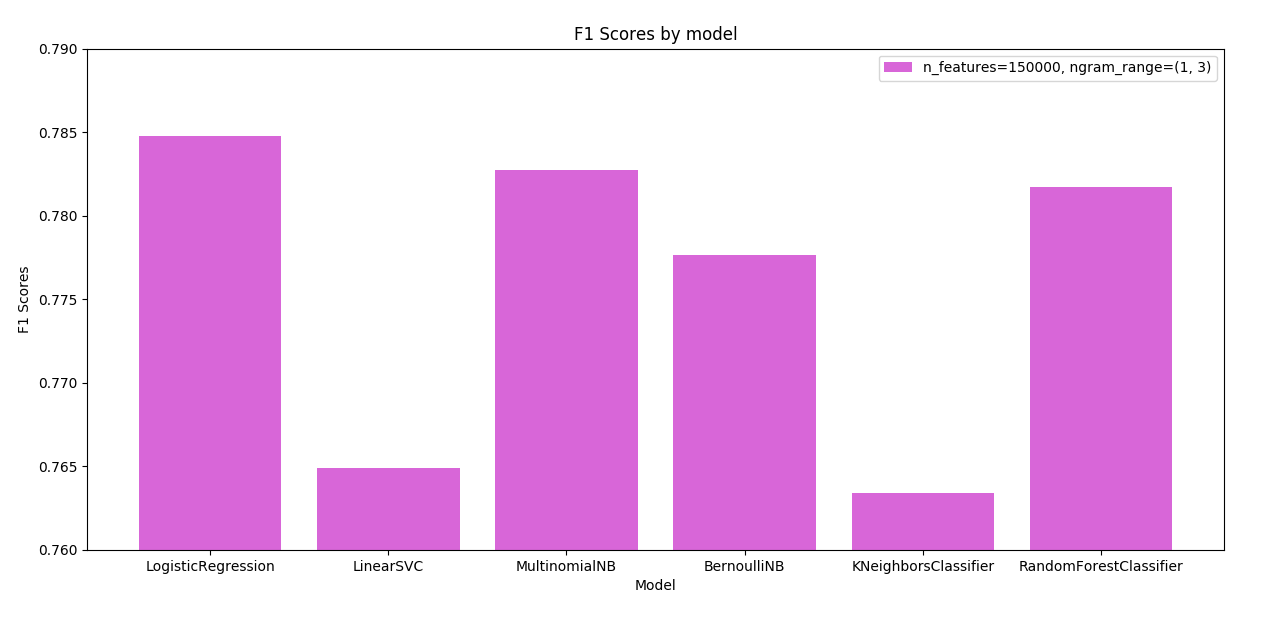
\includegraphics[scale=0.5]{graphs/models.png}
\label{model:graph}
\end{figure}

The inbuilt models in the sklearn package with default settings were used for initial comparison, and as we can see from Figure \ref{model:graph} the difference between the models is very slight, with the F1 scores all within a 3\% range of score. Since each of the models compared are all using their default settings within the sklearn package, more work could be done to optimise them further in the future, but just to argue for choosing the best default classifier the following hypothesis test is run.

\subsubsection{Hypothesis Tests}

As expected logistic regression leads to the highest results, but to be certain we run a hypothesis test to ensure the F1 score is greater than the next highest result, Multinomial Naive Bayes as follows:

$$ H_0: \textnormal{F1 score for the Logistic Regression is the same as Multinomial NB}$$
$$ H_a: \textnormal{F1 score for the Logistic Regression is the greater than Multinomial NB}$$

Using the Wilcoxon rank sum test with 90\% confidence interval, p = 0.02 so reject $H_0$.

We can select Logistic Regression as the optimal classification model to use.


\subsection{Oversampling and Undersampling}

To carry out the investigation of applying the oversampling and undersampling methods, the library functions in the imblearn API is used, which can be used in conjunction with the sklearn methods easily. 

Since it is unclear whether these methods will actually improve the model, comparing against the model that we already have is necessary, and as we can see from the results from the investigation shown in  Figure \ref{oversamplegraph}, using any of the oversampling methods decreases the F1 score by a significant amount. 

\begin{figure}[ht]
\caption{Graph showing the F1 score for different oversampling methods}
\centering
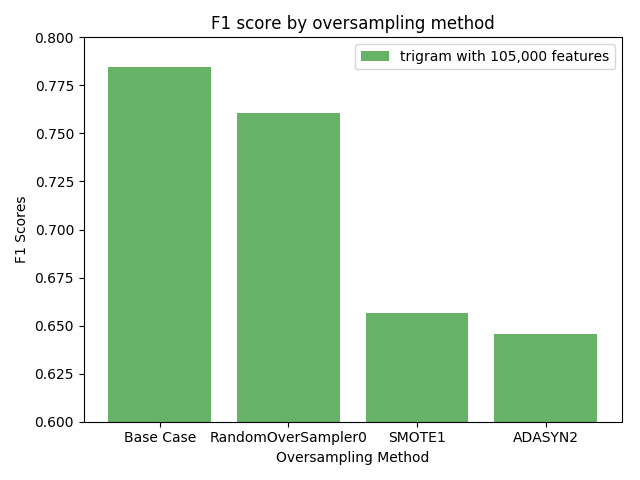
\includegraphics[scale=0.7]{graphs/oversampling.png}
\label{oversamplegraph}
\end{figure}

An explanation as to why this is happening is most likely a combination of using textual data, which is known to cause issues with oversampling methods, and the severity of the imbalance in the data. In the valence class, which is the one we are analysing at this point, the negative samples make up less than 10\% of the overall data and therefore many of the synthetic samples that are created will not make grammatical sense and be of poor quality. 


The undersampling methods were known to not give promising results, but due to the issues with oversampling over such a large class imbalance, briefly investigating this was something that could potentially have worked, but as the experimental results shown in Figure \ref{undersamplegraph}, they all made the model perform significantly worse and hence can be disregarded.

\begin{figure}[ht]
\caption{Graph showing the F1 score for different undersampling methods}
\centering
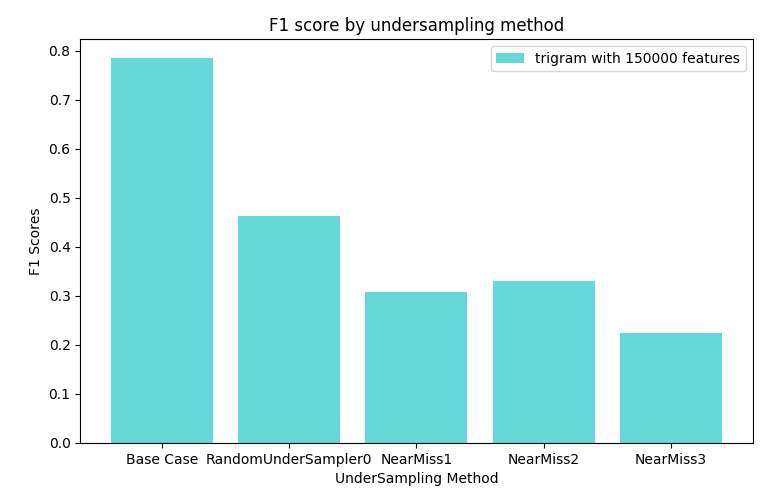
\includegraphics[scale=0.6]{graphs/undersample.png}
\label{undersamplegraph}
\end{figure}

\pagebreak

\subsection{Final Model}

The final model that was produced then had the following characteristics: 

\begin{itemize}
    \item The data was formatted into trigram tokens.
    \item The most frequent 105,000 n-gram tokens were used as input features.
    \item The classification model is Logistic Regression.
    \item No oversampling or undersampling techniques were applied.
\end{itemize}

Which results in a model that has the F1 scores for the prediction of each dimension shown in Table \ref{ML:f1}.

\begin{table}
\centering
\label{ML:f1}
\caption{F1 scores for the 3 dimensions for machine learning model}
\begin{tabular}{ |p{3cm}|p{3cm}|}
 \hline
  Dimension & F1 Score \\
 \hline
  Valence & 0.78\\
  Arousal & 0.86 \\
  Dominance & 0.89\\
 \hline
\end{tabular}

\end{table}

\subsection{Implementation}

The simplest solution to provide an interface between the final produced semantic prediction model and the Spotify API is to create a web application. The final classification model was hosted on a very simple python server that takes text as an input, and returns whether it classes the text as Positive, Negative or Neutral for each of the Valence, Arousal or Dominance dimensions. 

The final solution, as shown in Figure \ref{implementationLayout}, consists of three distinct hosted solutions, two of which access the API hosted by Spotify to access song data and authentication the user to allow their top songs to be obtained.

The UI was chosen to be built in Angular.js and the music API with Node.js due to prior development knowledge, and hence ease of prototyping. 
To ensure that any resultant song given back was one that the user could relate to, the final song is taken from a selection of the users recent top songs, which they allow the application access to through the authentication process.
The music API, built in Node.js is influenced by the structure of existing Spotify API projects \cite{moodtape}, and is built mostly using the Node package spotify-web-api-node \cite{nodeSpotify}.

\begin{figure}[ht]
\caption{General layout of how the web application is structured.}
\centering
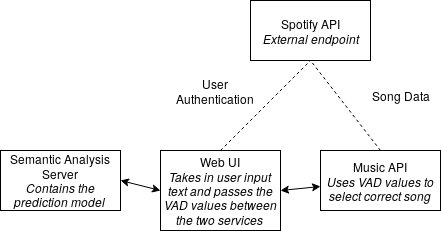
\includegraphics[scale=0.6]{litImgs/interfaceLayout.png}
\label{implementationLayout}
\end{figure}

Choosing how to relate the VAD values to the data returned for the songs was relatively arbitrary, and something that if there was more time could be investigated further. Since the song data returns a Valence value for the song it is obvious to map those two attributes together, and it was chosen to map the Arousal to the "Energy" attribute, and the Dominance to the "Danceability", but this is something that can be improved upon.

The main goal of the implementation is to attempt to relate an emotion in text, which is subjective, to a song since that is also subjective.

A decision was made to not show the user the VAD values, and just the result song to begin with. After the users reaction to the response song has been assessed, the calculated Ekmans emotion can be shown (calculated by the figures given in Table \ref{ekmansTable}) and discussed. \todo{this will be written about in the Results and discussion section}

\begin{figure}[ht]
\caption{User activity through the application}
\centering
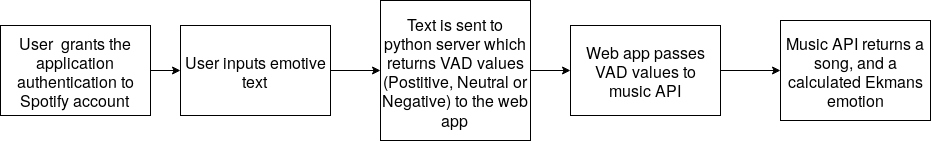
\includegraphics[scale=0.6]{litImgs/interfaceFlow.png}
\label{implementationLayout}
\end{figure}

\begin{figure}[ht]
\caption{Layout of main UI page}
\centering
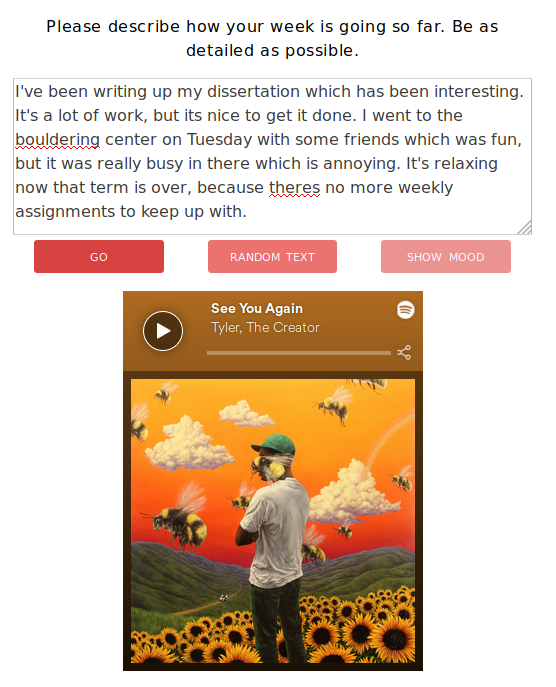
\includegraphics[scale=0.4]{implementation/tamara.png}
\label{UIlayout}
\end{figure}

